% Este archivo es parte de la memoria del proyecto fin de carrera
% de Manuel López Urbina. Protegida bajo la licencia GFDL.
% Para más información, la licencia completa viene incluida en el
% fichero fdl-1.3.tex

% Copyright (C) 2017 Manuel López Urbina

\newpage

\chapter{Comunicaciones}
\label{chap:comunicaciones}

En el presente capítulo comenzaremos con una introducción sobre el funcionamiento y los fundamentos teóricos sobre cómo se gestionan las diferentes conexiones y eventos de cualquier aplicación
Sails para, posteriormente, centrarnos específicamente en la descripción de un caso práctico desarrollado en el presente proyecto con la finalidad de comprender mejor su funcionamiento y poder afianzar
conocimientos.


\section{Introduccion}
\label{sec:fundamentos}

En esta sección se comenzaremos destacando aquellos aspectos teóricos sobre cómo Sails, framework Node JS utilizado en el desarrollo, trabaja con websocket y socket.io.\\

Como sabemos, un servidor http no puede enviar datos a menos que un cliente los haya solicitado mediante una petición. Los Websockets, en cambio, presentan la particularidad de que
permiten que un servidor envíe datos a un cliente sin la necesidad de que éstos sean solicitados, al menos de una manera inmediata. Estas solicitudes, realizadas con anterioridad, se formalizan mediante suscripciones, concepto que 
iremos constantemente haciendo referencia a lo largo del presente capítulo y que debemos recordar.\\


\begin{figure}%
    \centering
    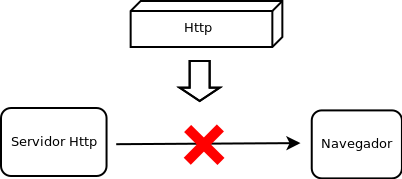
\includegraphics[width=7cm]{diagramas/http-weboscket.png}
    \qquad
    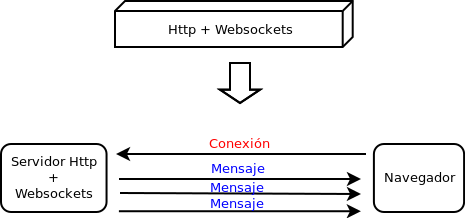
\includegraphics[width=7cm]{diagramas/http+weboscket.png}
    \caption{Peticiones entre un navegador y un servidor http con y sin el empleo de websockets.}%
    \label{fig:http-request}%
\end{figure}

Anteriormente comentamos que el servidor http no puede enviar datos a menos que el cliente lo haya solicitado y los Websockets permiten que un servidor envíe datos no solicitados una vez que se hace 
una conexión inicial (suscripción) desde el lado del cliente. Una aplicación Sails típica queda dividida en dos partes. La primera, en el lado del servidor, consta de un servidor http junto con un nodo
central que actúa como un servidor de sockets.\\ 

En segundo lugar, en el lado del cliente, se dispone de los diferentes códigos html y funciones JavaScript para realizar las conexiones con el servidor. Estas conexiones cliente-servidor permiten que 
cualquier otro cliente conectado pueda enviar mensajes al servidor para que a su vez éstos sean emitidos a los clientes que se encuentren conectados en la aplicación en ese instante.\\

Además cada socket posee un identificador único que identifica de manera inequívoca el cliente o, en nuestro, caso el navegador que está accediendo a la página.\\

Destacar también el concepto de salas o rooms de Socket.io. Las salas nos permite agrupar los sockets de modo que en lugar de mensajes que son enviados a todos los sockets conectados, se puede enviar mensajes
sólo a los sockets que están asociados con una sala. De esta podremos mandar mensajes específicos para un cliente concreto, todos ellos o un conjunto de los mismos. \\


\begin{figure}[H]
  \begin{center}
    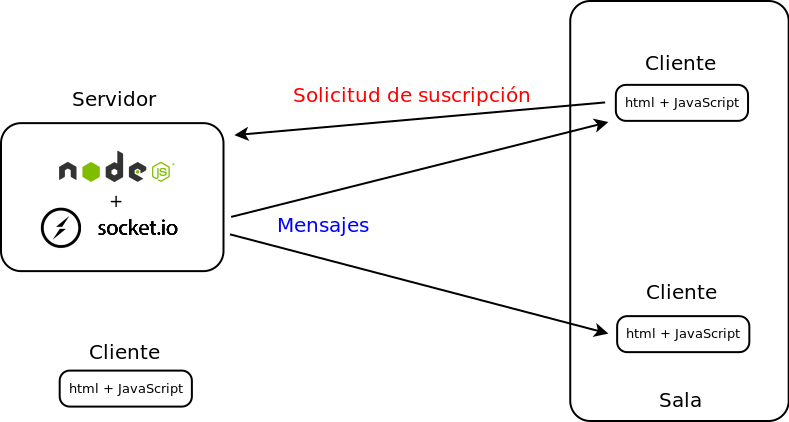
\includegraphics[scale=0.35]{diagramas/salas-websocket.png}
  \end{center}
  \caption{Representación de una sala compuesta por dos clientes.}
  \label{view:userindex}
\end{figure}


De todo los anterior podemos deducir que Sails es un framework especialmente potente, el cual proporciona infinidad de posibilidades a desarrollar. A continuación se cita un fragmento tal y 
como podemos extraer de la página oficial de Sails:\\

\begin{center}
\emph{Sails.js facilita el desarrollo de aplicaciones Node.js empresariales. Ha sido diseñado para imitar el patrón MVC de frameworks como Ruby on Rails, pero con soporte para los requisitos de aplicaciones modernas: data-driven APIs con una arquitectura escalable y service-oriented. Es especialmente bueno para el desarrollo de chats, cuadros de mando en tiempo real o juegos multijugadores.} 
\end{center}


En este caso menciona diferentes aplicaciones tipo que pueden desarrollarse con Sails, desde un chat, cuadros de mando en tiempo real o juegos multijugadores. RobotUI resulta como una combinación de las 
anteriores puesto que incorpora cuadros de mandos, sistema de mensajería y también es considerado como un juego ya que también está enfocado al entretenimiento.\\


\section{ Conexión y suscripción }
\label{sec:comunicaciones-robotui}

Tras la comprensión de los fundamentos descritos en el punto \ref{sec:fundamentos} donde se recogen los principios de comunicación con websockets pasamos
a trasladarlos a un caso práctico describiendo una de las funcionalidades del proyecto donde éstos son aplicados de tal manera que se facilite su comprensión.\\

Como sabemos, Sails nos ayuda a incorporar funcionalidades en tiempo real a nuestra aplicación web gestionando una serie de eventos aplicándolos sobre los modelos. Para el caso a describir nos
centraremos en el modelo \emph{Usuario} de RobotUI. Uno de los atributos de este modelo es un booleano \emph{online}, el cual representa si un usuario se encuentra logueado en el sistema o no.
El objetivo es saber cuando el usuario cambia el estado para poder proporcionar una actualización en tiempo real de la página de gestión de usuarios \ref{view:userindex} de manera que cuando usuario
inicie sesión o salga de la aplicación se alterne entre las imágenes online: \icontext{.2}{.35}{imagenes/comunicaciones/online.png} y offline: \icontext{.2}{.35}{imagenes/comunicaciones/offline.png} sin necesidad de refrescar la página manualmente.\\

\begin{figure}[H]
  \begin{center}
    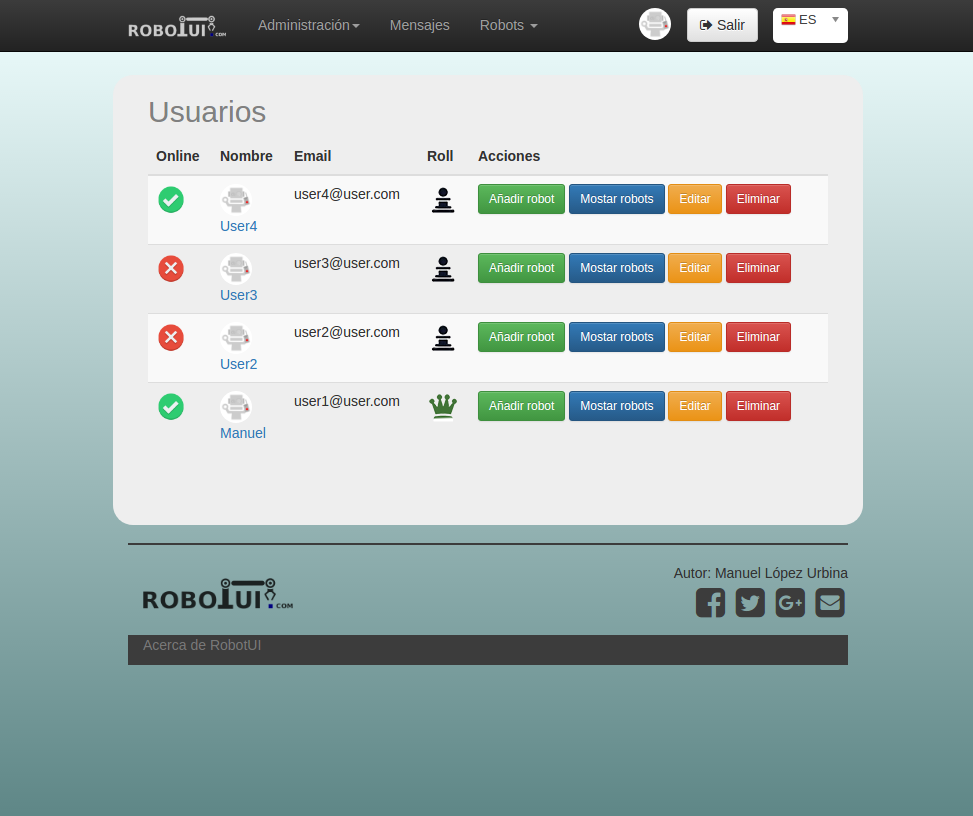
\includegraphics[scale=0.35]{imagenes/comunicaciones/index-usuarios.png}
  \end{center}
  \caption{Página de gestión de usuarios actualizable en tiempo real.}
  \label{view:userindex}
\end{figure}

Para capturar los eventos correspondientes al modelo \emph{Usuario} o cualquier otro debemos realizar una suscripción. Sails incorpora dos modalidades de suscripción. suscripción a clase y 
suscripción a modelo.\\

¿Cuál es la diferencia entre suscribirse a una ``clase'' frente a la suscripción a una ``instancia'' de un modelo? Al suscribirse a la ``clase'' del modelo, el socket podrá escuchar la creación de 
nuevas instancias de modelo mediante un método denominado publishCreate(). Mientras que la suscripción a ``instancia'' permite al socket escuchar los cambios de modelos a través de los métodos
publishUpdate y/o publishDestroy de una instancia o conjunto de instancias en concreto.\\


Por tanto, centrándonos en el ejemplo de los usuarios, debemos realizar la suscripción mediante la definición de una acción en el controlador de usuario. La acción se denominará \emph{user\_subscribe}.\\

En dicha acción podremos acceder al socket solicitante vía req.socket. Así que, primeramente se realiza una suscripción a la sala de ``clase'' del usuario mediante User.watch pasando 
req.socket como argumento. De esta manera nos hemos suscrito a la clase del modelo de usuario.\\

Seguidamente se realiza la suscripción a las instancias del modelo de usuario mediante el método User.subscribe pasando como parámetro el socket solicitante obtenido a través de req.socket seguido
de un segundo argumento, que se corresponde con las instancias existentes de usuarios. Las instancias de los usuarios existentes son recuperadas mediante un método de búsqueda para que, posteriormente, su salida 
sea pasada al método de suscripción como segundo argumento. Con esto ya nos hemos suscrito a las salas de instancias del modelo de usuario.\\

A continuación mostramos el código que realiza la suscripción al modelo Usuario en sus dos modalidades, suscripción a clase de modelo y suscripción a instancias de modelo descritas anteriormente:\\

\begin{lstlisting}[language=JavaScript]

  user_subscribe: function (req, res, next) {
    if (req.isSocket) {
      //Update, destroy...
      User.find(function foundUsers(err, users) {
        if (err) return res.badRequest(err);

        User.subscribe(req.socket, users);
      });

      //Create
      User.watch(req);
      console.log('User ' + req.session.User.id + 'with socket id ' + sails.sockets.id(req) + ' is now subscribed to the model class \'User\'.');
    } else {
      res.view();
    }
  }
  
\end{lstlisting}

Ahora bien, ya nos encontramos suscritos a un modelo, pero... ¿Qué ocurre con publishCreate, publishUpdate y publishDestroy?, ¿Dónde se realiza la llamada a estos métodos?\\


Para ello solamente debemos llamar al método en la acción deseada, por ejemplo, al crear una sesión, tan solo debemos actualizar el usuario como \emph{online} y mandar el mensaje correspondiente mediante
el método publishUpdate:\\

\begin{lstlisting}[language=JavaScript]

        //Cambio de estado a online
        User.update(user.id, {online: true, longitude: long, latitude: lat}, function (err){
          if (err) return next(err);

          //Informar a otros clientes (sockets abiertos) que el usuario esta logueado
          User.publishUpdate(user.id, {
            loggedIn: true,
            id: user.id
          });
         });

\end{lstlisting}

Tras ello se notificará a todos los clientes que han sido suscritos a las instancias del modelo Usuario de que un determinado usuario ha cambiado su estado.\\



Del mismo modo para \emph{publishCreate} o \emph{publishDestroy}.\\


¿Y desde el lado del cliente? ¿Cómo realizamos las llamadas a las diferentes acciones de suscripción y cómo capturamos los eventos?\\

Para la realización de las suscripciones y captura de eventos las siguientes funciones ejecutables en el cliente resultan de vital importancia.\\

Primeramente tenemos la función \emph{savesocket} la cual realiza la llamada al método saveSocketID del controlador \emph{Session}. Dicho método crea un registro en base de datos ligando el
identificador del socket abierto con el usuario que se encuentra identificado en el sistema, de tal manera que siempre sabremos qué socket corresponde con qué usuario. Este almacenamiento se debe
a que al realizarse una nueva conexión de un usuario en el sistema el servidor debe conocer y registrar a dicho cliente con la finalidad de seguir su comportamiento, sus acciones y movimientos por toda
la aplicación.\\

Dicho código JavaScript se encuentra localizado en el layout principal de la aplicación de tal manera que independientemente de qué vista resulte cargada siempre se ejecutará el siguiente fragmento
de código realizando el almacenamiento del socket abierto por el usuario:\\

\begin{lstlisting}[language=JavaScript]


<script type="text/javascript">

  $.when(savesocket()).done(function(){
    if (typeof subscribeAndListen == 'function') {
      subscribeAndListen();
    }
    listenMessages();
  });

  //Funcion para tener en to do momento almacenado en la tabla session los sockets conectados junto con el usuario al que pertenece
  function savesocket() {
    io.socket.get("/session/saveSocketID");
  }
</script>

\end{lstlisting}


Función saveSocketID, la cual es llamada en cliente y que se encuentra implementada en el controlador \emph{session} en el lado del servidor. Esta función realiza el registro de un nuevo cliente en
la base de datos tras recibir el identificador correspondiente al nuevo socket creado.\\

El código inferior muestra la implementación en el lado del servidor de la función saveSocketID:\\

\begin{lstlisting}[language=JavaScript]


  //Almacenamiento en la base de datos la sesion de cada usuario de la pagina
  saveSocketID: function(req, res) {
    if (!req.isSocket) return res.badRequest();

    var socketId = sails.sockets.id(req);
    // => "BetX2G-2889Bg22xi-jy"

    var sessionObj = {
      socket_id: socketId,
      user_id: req.session.User != undefined ? req.session.User.id : null
    };

    Session.create(sessionObj).exec( function (err, session) {
      if (err) return res.badRequest();

      console.log('\n................................................');
      console.log('Conectando a Sails js...');
      console.log('Cliente conectado - id del socket: ' + socketId);
      console.log('..................................................');

      return;
    });
  }
  
\end{lstlisting}

Una vez tenemos almacenado el par socket-usuario en base de datos buscamos la función subscribeAndListen, la cual será específica según la vista en la que nos encontremos, por ejemplo, si nos encontramos en el panel
de administración de usuarios, la función subscribeAndListen será específicaespecífica para cada funcionalidad que queramos inicializar o a qué eventos nos deseemos suscribir. Si nos encontramos en la vista de índice de robots, la función se suscribirá 
a los eventos de conexión y desconexión de robots. O si estamos visualizando el funcionamiento de un robot entonces la función capturará los eventos que se correspondan con la captación de los diferentes comandos o datos transmitidos.\\

En el código inferior mostramos la función subscribeAndListen que implementa la suscripción a los eventos correspondiente a la conexión, desconexión y borrado de usuarios del panel de
administración descrito en el apartado \ref{sec:fundamentos}. Esta función está localizada en el partial que implementa la vista correspondiente con el citado panel:\\

\begin{lstlisting}[language=JavaScript]


<script type="text/javascript">

  function subscribeAndListen() {
    io.socket.get('/user/user_subscribe');

    io.socket.on('user', function (obj) {
      if (obj.verb == 'created') {
        var user = obj.data;
        $.ajax({
          url: '/user/render',
          type: 'GET',
          data: {id: user.id},
          success: function(data){
            $("#user_list").append(data);
           toastr.info('<%= i18n('user_created')%>', 'RobotUI' )
          }
        });
      }

      if (obj.verb == 'updated') {
        var data = obj.data;
        change_img_state(data.id, data.loggedIn, '<%= i18n('connect')%>', '<%= i18n('disconnect')%>');

        if (data.id != '<%= req.session.User.id %>') {
          if (data.loggedIn) {
           toastr.info('<%= i18n('user_connected')%>', 'RobotUI');
          } else {
           toastr.info('<%= i18n('user_disconnected')%>', 'RobotUI');
          }
          console.log('User has been updated to online:' + data.loggedIn);
        }
      }

      if (obj.verb == 'destroyed') {
        $("#user_" + obj.id).remove();
       toastr.info('<%= i18n('user_destroyed') %>', 'RobotUI' );
      }

    });

  }

</script>

\end{lstlisting}


Por otro lado se realiza la llamada a la función \emph{listenMessages} ya que independientemente de la vista en la que nos encontremos siempre nos mantendremos a la escucha de los mensajes 
recibidos a nuestra bandeja de entrada por parte de otros usuarios.\\

\begin{lstlisting}[language=JavaScript]

  //Evento a la espera de recibir mensajes y notificar al usuario
  function listenMessages(){
    io.socket.on('user', function messageReceived(message) {
      switch (message.verb) {
        case 'messaged':
          var pathname = window.location.pathname;
          if(pathname == '/message/index'){
            location.reload();
          }else{
            new_msg_num_update('<%= i18n('messages') %>');
          }
          toastr.info('<%= i18n('new_message')%>' + '<a href="/message/index"> <%= i18n('open_here')%> </a>' , 'RobotUI');
          break;
        default:
          break;
      }
    });
  }
\end{lstlisting}



\section { Desconexión }
\label{sec:deconexion}

En este apartado describiremos los puntos de mayor relevancia a la hora de la desconexión de alguna de las diferentes comunicaciones establecidas comenzando con la desconexión de un usuario.\\

Cuando un usuario realiza una desconexión, bien deslogueándose de la página o cerrando una de las ventanas abiertas, automáticamente se lanza una llamada a la 
función \emph{afterDisconnect} localizada en el fichero \emph{config/Socket.js} del servidor. Función que será ejecutada cada vez que un socket es desconectado del sistema.\\

Dicha función primeramente localiza qué sesión en la base de relacionada está relacionada con identificador del socket desconectado. Si este socked estaba usando algún robot, éste se libera cambiando el estado
del robot a \emph{libre}. Y se informa a todos los sockets abiertos que el robot queda libreado y accesible al resto de usuarios.\\

\begin{lstlisting}[language=JavaScript]
  Robot.update({id: session.robot_id}, {busy: false}, function robotUpdated(err) {
    if (err) return next(err);

    //Informar a otros clientes (sockets abiertos) que el robot queda liberado
    Robot.publishUpdate(session.robot_id, {
      busy: false,
      id: session.robot_id
    });
  });
\end{lstlisting}


A continuación, se comprueba si el usuario no dispone de más sockets abiertos. Si fuera el caso de que no los disponga, entonces se procede a cambiar su estado a desconectado y se emite o se informa al resto de clientes (sockets abiertos)
que el usuario ya no se encuentra en el sistema. Llamada al método \emph{User.publishUpdate}: \\

\begin{lstlisting}[language=JavaScript]
   User.publishUpdate(session.user_id, {
    loggedIn: false,
    id: session.user_id
  });
\end{lstlisting}


Se comprueba si el usuario desconectado se encontraba en alguna \emph{room}. Pongamos como ejemplo que el usuario ha abandonado la visualización de un robot por lo queda
se debe informar a todos los sockets integrantes de esa \emph{room} que un usuario con un identificador determinado la ha abandonado con la función \emph{ sails.sockets.broadcast }.
A continuación se muestra el fragmento de código:\\

\begin{lstlisting}[language=JavaScript]

//Emite a cada room que que se encuentre la sesión que un usuario la ha abandonado
session.rooms.forEach(function (room) {
  sails.sockets.broadcast(room.room_name, {type: 'exit', msg: {user_id: session.user_id}});
});

\end{lstlisting}

Finalmente se destruye la sesión:\\

\begin{lstlisting}[language=JavaScript]
    Session.destroy(session.id, function sessionDestroyed(err) {
      if (err) return cb();
      return cb();
    });
\end{lstlisting}


A continuación mostramos el código completo de la función \emph{afterDisconnect}:\\


\begin{lstlisting}[language=JavaScript]

  afterDisconnect: function(session, socket, cb) {
     console.log('Cliente desconectado - id del socket: ' + socket.id);

    //Session del socket cerrado,
    Session.findOne({socket_id: socket.id}).populate('rooms').exec(function (err, session) {
      if (err) return cb();
      if (!session) return cb();

      //Comprobar si el soscket estaba usando algun robot para liberarlo:
      if (session.robot_id) {
        console.log('Socked was using a robot');

        Robot.update({id: session.robot_id}, {busy: false}, function robotUpdated(err) {
          if (err) return next(err);

          //Informar a otros clientes (sockets abiertos) que el robot queda liberado
          Robot.publishUpdate(session.robot_id, {
            busy: false,
            id: session.robot_id
          });
        });
      }


      //Emite a cada room que que se encuentre la sesión que un usuario la ha abandonado ->  
      session.rooms.forEach(function (room) {
        sails.sockets.broadcast(room.room_name, {type: 'exit', msg: {user_id: session.user_id}});
      });


      //Comprobar si el usuario tiene más sockets abiertos:
      Session.count({user_id: session.user_id}).exec(function countUserSessions(error, n_sessions) {
        console.log('There are ' + n_sessions + ' users ' + session.user_id);

        //Cambiamos el usuario a offline si solo tenía una ventana o conexión abierta.
        if (n_sessions == 1) {
          User.update(session.user_id, {online: false}, function (err) {
            if (err) return cb(err);

            //Informar a otros clientes (sockets abiertos) que el usuario ya NO se encuentra logueado
            User.publishUpdate(session.user_id, {
              loggedIn: false,
              id: session.user_id
            });
          });
        }

        Session.destroy(session.id, function sessionDestroyed(err) {
          if (err) return cb();
          return cb();
        });
      });
    });
  }

\end{lstlisting}
  
 
 En este punto ya conocemos cómo la aplicación RobotUI gestiona las diferentes conexiones y cómo se realiza el almacenamiento en base de datos de la información necesaria para determinar qué sockets se 
 corresponde con qué usuarios en todo momento. Todo ello además ha sido explicado para la gestión de conexiones y desconexiones de usuarios notificando los cambios de estados entre \emph{online} y \emph{offline}.\\
 
 Para la conexión y desconexión de los robots se aplica la metodología anterior de manera análoga. Pero... en el caso particular de los robots. ¿Cómo se realizan las 
 comunicaciones entre el cliente (navegador) y el robot?, ¿Cómo es controlado un robot?, ¿Cómo se difunden los comandos lanzados a un robot al resto de usuarios espectadores?. En los sucesivos puntos iremos describiendo cómo se ha implementado estos
 comportamientos.\\
 
  
\section{Envío de comandos al robot}
  
  Cuando un usuario ha recibido la notificación de que un determinado dispositivo se encuentra disponible, entonces procede a acceder a su interfaz de control realizándose una conexión con el mismo.  Una vez establecida 
  dicha conexión el usuario puede proceder al lanzamiento de comandos para el control del robot. En ese momento se realiza un procedimiento para el envío de la información que consta de tres puntos:
    
 \begin{enumerate}
  \item Envío del comando indicado al robot.\\
  \item Envío de notificación al servidor del comando lanzado. 
  \item Envío de la notificación por parte del servidor a todos los clientes suscritos al robot de que un comando ha sido enviado.
 \end{enumerate}

 EL gráfico \ref{diagram:conexiones-controlador} muestra el flujo de datos generado cada vez que un comando es envíado al robot:
 
\begin{figure}[H]
  \begin{center}
    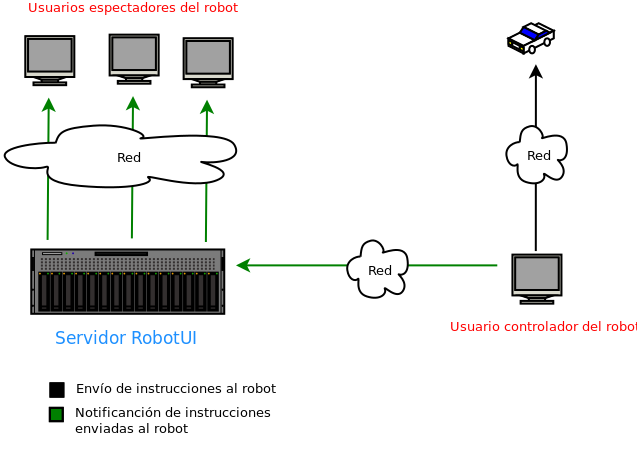
\includegraphics[scale=0.5]{diagramas/flujo_comunicaciones_controlador.png}
  \end{center}
  \caption{Esquema representativo del flujo de datos originado por un usuario controlador de un robot.}
  \label{diagram:conexiones-controlador}
\end{figure}
 
  
El código inferior realiza el envío del comando al robot para su interpretación y al servidor para su posterior difusión a los clientes suscritos:\\
 
 \begin{lstlisting}[language=JavaScript]
 
    //Presionar boton accion!
    $('[id^=button_]').click(function (e) {
      e.preventDefault();
      var button_pressed_id = this.id.replace('button_custom_','');
      var code = document.getElementById(this.id).value

      //Comunicación al servidor del comando para difundir a los usuarios espectadores
      io.socket.get('/interface/emit_action/',{robot: '<%=robot.id %>', id: button_pressed_id, msg: code })

      if (code != ''){
        $('#chat').prepend('- ' + code + '<br/>');
        //Mandar instruccion al robot
        socket.emit('action', code);
        console.log('Emitiendo comando: ' + code );
      }
    });

 \end{lstlisting}
 
 
\section{Captura de datos del robot}

 Ahora bien, ya sabemos el procedimiento realizado a la hora de lanzar comandos al robot pero, esta comunicación tendría poco sentido si no capturamos sus respuestas. Estas respuestas pueden ser los datos correspondientes
 a los diferentes frames obtenidos por la cámara de vídeo del robot o aquellos datos correspondientes a la medición de los diferentes sensores de los que pueda disponer el robot.

 
 \begin{figure}[H]
  \begin{center}
    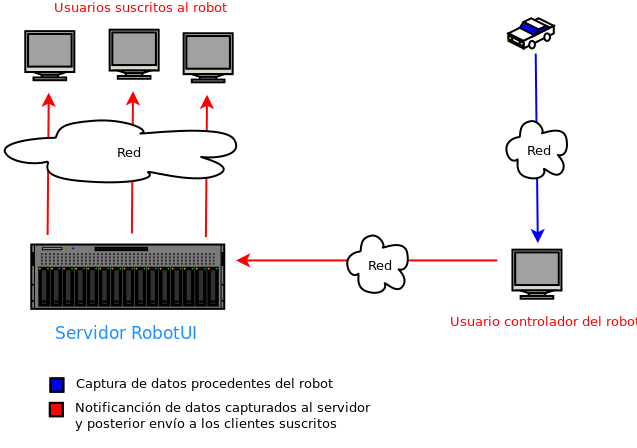
\includegraphics[scale=0.5]{diagramas/flujo_comunicaciones_captura.png}
  \end{center}
  \caption{Esquema representativo del flujo de datos originado por un usuario controlador de un robot tras la captura de datos procedentes del robot.}
  \label{diagram:conexiones-controlador}
\end{figure}
 
 
 El código inferior se corresponde con el evento lanzado cada vez que un frame de vídeo es capturado. Dicho código envía al servidor el frame para su postreior difusión y ``dibuja'' los datos capturados en el canvas de la interfaz:\\
 
 
\begin{lstlisting}[language=JavaScript] 
    //Captura de video
    socket.on('<%= video.event_name %>', function(data) {
      io.socket.get('/interface/emit_video/',{robot: '<%=robot.id %>', id: '<%= video.id %>', msg: data });
      draw_image_to_canvas('play_<%= video.id %>', data)
    });
\end{lstlisting}


Código de la acción \emph{emit\_video}, la cual emite el frame capturado a todos los clientes que se encuentran suscritos al robot (broadcast a todos los clientes suscritos a la sala cuyo nombre se
corresponde con el identificador del robot):\\

\begin{lstlisting}[language=JavaScript] 
  //Emision de las acciones a los vivitantes de una interfaz
  emit_video: function(req, res){
    if (!req.isSocket) return res.badRequest();
    sails.sockets.broadcast(req.param('robot'), {type: 'video', id: req.param('id'), msg: req.param('msg')});
  },
\end{lstlisting}



